% ============================================================
%  DISCOVERY CURRICULUM — Journey 2, Module 4
%  "Shape, Optimisation, and Motion"
%  Compile with: pdflatex J2_M4.tex  (run twice for references)
% ============================================================

\documentclass[12pt, a4paper]{article}

\usepackage[a4paper, top=2.5cm, bottom=2.5cm, left=2.8cm, right=2.8cm, headheight=15pt]{geometry}
\usepackage{amsmath, amssymb, amsthm}
\usepackage{xcolor}
\usepackage{mdframed}
\usepackage{enumitem}
\usepackage{tikz}
\usetikzlibrary{arrows.meta, positioning, calc}
\usepackage{pgfplots}
\pgfplotsset{compat=1.18}
\usepackage{booktabs}
\usepackage{fancyhdr}
\usepackage{titlesec}
\usepackage{parskip}
\usepackage{hyperref}
\hypersetup{colorlinks=true, linkcolor=NavyBlue, urlcolor=NavyBlue}

% ── Colours ─────────────────────────────────────────────────
\definecolor{NavyBlue}{HTML}{1A3A5C}
\definecolor{MidBlue}{HTML}{2E6DA4}
\definecolor{Gold}{HTML}{C8922A}
\definecolor{LightBlue}{HTML}{EBF2FA}
\definecolor{LightGold}{HTML}{FDF4E3}
\definecolor{DarkGrey}{HTML}{3A3A3A}
\definecolor{BoxGreen}{HTML}{E8F5E9}
\definecolor{SidebarGrey}{HTML}{F5F5F5}

% ── Section formatting ───────────────────────────────────────
\titleformat{\section}{\Large\bfseries\color{NavyBlue}}{}{0em}{}[{\color{MidBlue}\vspace{2pt}\rule{\linewidth}{1.5pt}}]
\titleformat{\subsection}{\large\bfseries\color{MidBlue}}{}{0em}{}

% ── Header / Footer ─────────────────────────────────────────
\pagestyle{fancy}
\fancyhf{}
\fancyhead[L]{\small\color{DarkGrey}\textit{Discovery Curriculum}}
\fancyhead[R]{\small\color{DarkGrey}\textit{Journey 2 $\cdot$ Module 4}}
\fancyfoot[C]{\small\color{MidBlue}\thepage}
\renewcommand{\headrulewidth}{0.4pt}

% ── Environments ─────────────────────────────────────────────
\newmdenv[
  backgroundcolor=NavyBlue!7,
  linecolor=NavyBlue, linewidth=2pt,
  leftline=true, rightline=false, topline=false, bottomline=false,
  innerleftmargin=14pt, innerrightmargin=10pt,
  innertopmargin=10pt, innerbottommargin=10pt,
  skipabove=14pt, skipbelow=10pt
]{puzzlebox}

\newmdenv[
  backgroundcolor=LightGold,
  linecolor=Gold, linewidth=2pt,
  leftline=true, rightline=false, topline=false, bottomline=false,
  innerleftmargin=14pt, innerrightmargin=10pt,
  innertopmargin=10pt, innerbottommargin=10pt,
  skipabove=14pt, skipbelow=10pt
]{discoverybox}

\newmdenv[
  backgroundcolor=LightBlue,
  linecolor=MidBlue, linewidth=1.5pt,
  roundcorner=4pt,
  innerleftmargin=14pt, innerrightmargin=10pt,
  innertopmargin=10pt, innerbottommargin=10pt,
  skipabove=14pt, skipbelow=10pt
]{namebox}

\newmdenv[
  backgroundcolor=BoxGreen,
  linecolor=DarkGrey!35, linewidth=1pt,
  roundcorner=4pt,
  innerleftmargin=14pt, innerrightmargin=10pt,
  innertopmargin=10pt, innerbottommargin=10pt,
  skipabove=14pt, skipbelow=10pt
]{reflectionbox}

\newmdenv[
  backgroundcolor=SidebarGrey,
  linecolor=Gold, linewidth=1.2pt,
  leftline=true, rightline=false, topline=false, bottomline=false,
  innerleftmargin=12pt, innerrightmargin=10pt,
  innertopmargin=7pt, innerbottommargin=7pt,
  skipabove=10pt, skipbelow=10pt
]{thought}

\newcounter{problem}
\newenvironment{problem}[1][]{%
  \refstepcounter{problem}%
  \par\vspace{6pt}%
  \noindent\textbf{\color{MidBlue}Problem \theproblem}%
  \ifx&#1&\else\ \textit{(#1)}\fi\textbf{.}\enskip
}{\par\vspace{4pt}}

\newcounter{deepproblem}
\newenvironment{deepproblem}[1][]{%
  \refstepcounter{deepproblem}%
  \par\vspace{6pt}%
  \noindent\textbf{\color{NavyBlue}$\bigstar$\ Deep Problem \thedeepproblem}%
  \ifx&#1&\else\ \textit{(#1)}\fi\textbf{.}\enskip
}{\par\vspace{4pt}}

% ============================================================
\begin{document}
% ============================================================

\thispagestyle{empty}
\begin{center}
{\small\color{MidBlue}\textbf{DISCOVERY CURRICULUM}\quad$\cdot$\quad\textbf{JOURNEY 2: CHANGE}}

\vspace{0.6cm}
{\color{NavyBlue}\rule{\linewidth}{2pt}}
\vspace{0.5cm}

{\Huge\bfseries\color{NavyBlue}Module 4}\\[0.3cm]
{\LARGE\bfseries\color{MidBlue}Shape, Optimisation, and Motion}\\[0.4cm]
{\color{Gold}\rule{0.4\linewidth}{1.2pt}}\\[0.4cm]
{\large\itshape\color{DarkGrey}
The derivative does not just tell you how fast.\\[0.15cm]
It tells you the entire story of a function's shape.}

\vspace{1cm}
\begin{tabular}{rl}
\color{DarkGrey}\textbf{Journey}           & Journey 2 --- Change \\[4pt]
\color{DarkGrey}\textbf{Module}            & 4 of 6 \\[4pt]
\color{DarkGrey}\textbf{Prerequisites}     & J2 Modules 1--3 \\[4pt]
\color{DarkGrey}\textbf{You will discover} & Mean Value Theorem, curve sketching, optimisation, related rates, L'H\^{o}pital \\[4pt]
\color{DarkGrey}\textbf{Format}            & 8 problems $+$ 3 deep problems $\approx$ 13 pages \\
\end{tabular}

\vspace{1cm}
{\color{NavyBlue}\rule{\linewidth}{2pt}}
\end{center}

\vspace{0.5cm}

\noindent\textbf{What derivatives reveal about shape.}
You now know how to compute derivatives and integrals. This module asks what they \emph{tell} you --- not about instantaneous rates, but about the global character of a function. Where does it rise and fall? Where are its peaks and troughs? How does it bend? Where does it level off? And how do you use derivatives to find the best value of a quantity subject to constraints? These are the questions that make calculus indispensable in physics, engineering, and economics.

\newpage

% ============================================================
\section{Part 1 \texorpdfstring{---}{--} The Puzzle}
% ============================================================

\begin{puzzlebox}
\textbf{The Opening Puzzle.}

A farmer has 120 metres of fencing and wants to enclose a rectangular field. One side of the field is along a river and needs no fencing.

\medskip
\textbf{Question 1.} Write the area $A$ as a function of the side perpendicular to the river. What is the domain?

\textbf{Question 2.} Sketch $A$ as a function of this variable. Where does it appear to be maximised?

\textbf{Question 3.} Without calculus: by symmetry or AM-GM, find the maximum. Note how much work the calculus approach saves by making the method systematic and generalisable.

\textbf{Question 4.} At the maximum, what is $A'$? Does this always have to be true at a maximum inside the domain?
\end{puzzlebox}

% ============================================================
\section{Part 2 \texorpdfstring{---}{--} Exploration}
% ============================================================

\subsection{Step 1: The Mean Value Theorem}

The most important theorem connecting the derivative to the global behaviour of a function is the Mean Value Theorem. You have been using its content implicitly; now you will see it stated precisely.

\begin{problem}
\label{prob:mvt}
\begin{enumerate}[label=(\alph*), topsep=2pt]
  \item A car travels from Nairobi to Nakuru, a distance of 160 km, in exactly 2 hours. Prove that at some moment during the journey, the car's instantaneous speed was exactly 80 km/h.
  \item State the general claim: if $f$ is continuous on $[a,b]$ and differentiable on $(a,b)$, there exists $c \in (a,b)$ such that $f'(c) = \dfrac{f(b)-f(a)}{b-a}$. Explain what this says geometrically.
  \item Use the MVT to prove: if $f'(x) = 0$ for all $x \in (a,b)$, then $f$ is constant on $[a,b]$.
  \item Use (c) to prove: if $F'(x) = G'(x)$ for all $x$, then $F(x) = G(x) + C$ for some constant. This finally justifies the $+C$ in antiderivatives.
  \item Use the MVT to prove that $|\sin a - \sin b| \leq |a - b|$ for all real $a, b$.
\end{enumerate}
\end{problem}

\begin{thought}
\textbf{The MVT is not obvious.}
The Mean Value Theorem seems obvious: of course the instantaneous rate equals the average rate \emph{at some point}. But the proof is not trivial --- it requires Rolle's Theorem, which in turn requires the extreme value theorem (a continuous function on a closed interval attains its maximum and minimum), which requires the completeness of $\mathbb{R}$. The chain of dependencies goes all the way back to the foundations of the real numbers. What feels intuitively obvious is actually resting on quite deep ground. This is a recurring pattern in mathematics: the seemingly obvious is often the hardest to prove rigorously.
\end{thought}

\subsection{Step 2: Reading shape from derivatives}

\begin{problem}
\label{prob:curve_sketch}
For each function, determine: intervals of increase/decrease, local maxima/minima, intervals of concavity, inflection points. Then sketch the graph.
\begin{enumerate}[label=(\alph*), topsep=2pt]
  \item $f(x) = x^3 - 3x$
  \item $g(x) = x^4 - 4x^3$
  \item $h(x) = \dfrac{x}{1+x^2}$
  \item $k(x) = xe^{-x}$ for $x \geq 0$
\end{enumerate}
For each, use the following procedure:
\begin{enumerate}[label=\roman*., noitemsep, topsep=2pt]
  \item Find $f'$: locate critical points ($f'=0$ or undefined), determine sign of $f'$
  \item Find $f''$: locate inflection points ($f''=0$ changes sign), determine concavity
  \item Check behaviour as $x \to \pm\infty$ and at domain boundaries
  \item Assemble into a sketch
\end{enumerate}
\end{problem}

\begin{center}
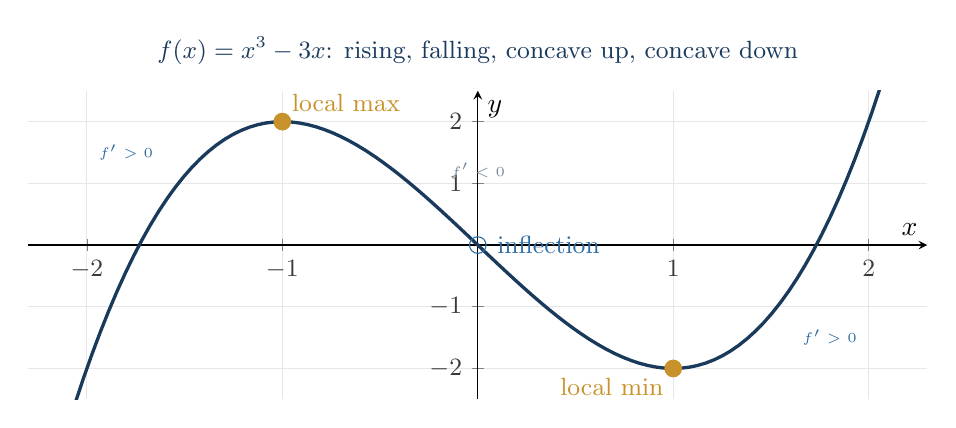
\begin{tikzpicture}
\begin{axis}[
  width=13cm, height=5.5cm,
  axis lines=center,
  xlabel={$x$}, ylabel={$y$},
  xmin=-2.3, xmax=2.3, ymin=-2.5, ymax=2.5,
  xtick={-2,-1,1,2}, ytick={-2,-1,1,2},
  tick label style={font=\small, color=DarkGrey},
  grid=major, grid style={DarkGrey!12},
  title={\small\color{NavyBlue}$f(x)=x^3-3x$: rising, falling, concave up, concave down},
]
\addplot[NavyBlue, very thick, domain=-2.1:2.1, samples=100] {x^3 - 3*x};
% Critical points at x=-1 (local max) and x=1 (local min)
\addplot[only marks, mark=*, mark size=3pt, Gold] coordinates {(-1,2)(1,-2)};
% Inflection at x=0
\addplot[only marks, mark=o, mark size=3pt, MidBlue] coordinates {(0,0)};
\node[Gold, font=\small, above right] at (axis cs:-1,2) {local max};
\node[Gold, font=\small, below left] at (axis cs:1,-2) {local min};
\node[MidBlue, font=\small, right] at (axis cs:0.05,0) {inflection};
% f' sign annotations
\node[font=\tiny, color=MidBlue] at (axis cs:-1.8, 1.5) {$f'>0$};
\node[font=\tiny, color=NavyBlue!60] at (axis cs:0, 1.2) {$f'<0$};
\node[font=\tiny, color=MidBlue] at (axis cs:1.8, -1.5) {$f'>0$};
\end{axis}
\end{tikzpicture}
\end{center}

\begin{thought}
\textbf{Concavity and the second derivative.}
The second derivative $f''$ measures how fast the slope is changing. Where $f'' > 0$, the slope is increasing --- the curve bends upward like a bowl ($\cup$). Where $f'' < 0$, the slope is decreasing --- the curve bends downward like an arch ($\cap$). An inflection point is where the concavity reverses. In economics, inflection points in cost functions mark the transition from \emph{increasing returns to scale} to \emph{decreasing returns to scale}. In physics, inflection points in potential energy curves locate unstable equilibria. The second derivative is not just a mathematical curiosity --- it identifies qualitative changes in a system's behaviour.
\end{thought}

\subsection{Step 3: Optimisation}

\begin{problem}
\label{prob:optimise}
\begin{enumerate}[label=(\alph*), topsep=2pt]
  \item \textbf{Can packaging.} A cylindrical tin must hold $500\,\text{cm}^3$. Find the dimensions (radius $r$, height $h$) that minimise the total surface area (two discs plus the curved side). Set up the constraint, eliminate one variable, then differentiate.
  \item \textbf{Snell's law.} Light travels from a point $A$ in a medium with speed $c_1$ to a point $B$ in a medium with speed $c_2$, crossing a flat interface. The light bends at the interface. Show that the path that minimises travel time satisfies $\dfrac{\sin\theta_1}{c_1} = \dfrac{\sin\theta_2}{c_2}$, where $\theta_1$ and $\theta_2$ are the angles to the normal. This is Snell's law of refraction.
  \item \textbf{Nearest point.} Find the point on the parabola $y = x^2$ closest to the point $(3, 0)$.
  \item \textbf{Profit maximisation.} A company sells $q$ units at price $p(q) = 50 - 0.1q$ (KES). The cost is $C(q) = 200 + 10q$. Find the quantity that maximises profit. What price does this correspond to?
\end{enumerate}
\end{problem}

\begin{thought}
\textbf{Fermat's principle and the unity of physics.}
Snell's law was known empirically before calculus. But its \emph{derivation} via minimisation --- Fermat's principle of least time --- revealed something profound: the path of light is not arbitrary, it is the path that extremises a quantity. This is a special case of a much deeper principle. In classical mechanics, the path of every particle is the one that extremises the \emph{action} (a quantity involving kinetic and potential energy integrated over time). In optics, quantum mechanics, electromagnetism, and general relativity, the laws of physics can be stated as: \emph{nature extremises something}. This principle --- the principle of least action --- is perhaps the deepest single idea in all of physics, and it rests on calculus. You will encounter it in Journey~4.
\end{thought}

\subsection{Step 4: Related rates}

\begin{problem}
\label{prob:related_rates}
Two quantities both depend on time. Differentiating a geometric or physical relationship with respect to time connects their rates of change.

\begin{enumerate}[label=(\alph*), topsep=2pt]
  \item A ladder of length 5 m leans against a wall. The base slides away from the wall at $0.5\,\text{m/s}$. How fast is the top sliding down when the base is 3 m from the wall?
  \item A spherical balloon is being inflated at $100\,\text{cm}^3/\text{s}$. How fast is the radius increasing when the radius is 10 cm?
  \item Two ships leave a port at noon. Ship A travels north at 20 km/h; ship B travels east at 15 km/h. How fast is the distance between them increasing at 2 pm?
  \item A conical tank (vertex down, half-angle $30°$) drains at $2\,\text{m}^3/\text{min}$. How fast does the water level fall when the depth is 4 m?
\end{enumerate}
For each: draw a diagram, name the variables, write the geometric/physical relationship, differentiate both sides with respect to $t$, substitute the known values.
\end{problem}

\subsection{Step 5: Indeterminate forms and L'H\^{o}pital's rule}

\begin{problem}
\label{prob:lhopital}
Some limits produce $\frac{0}{0}$ or $\frac{\infty}{\infty}$ directly. These are indeterminate forms.
\begin{enumerate}[label=(\alph*), topsep=2pt]
  \item Evaluate $\lim_{x\to 0}\dfrac{\sin x}{x}$ using the known fact that this limit equals 1. Verify numerically.
  \item \textbf{L'H\^{o}pital's rule}: if $\lim_{x\to a}f(x) = \lim_{x\to a}g(x) = 0$ (or both $\pm\infty$), and if $g'(a)\neq 0$, then $\lim_{x\to a}\frac{f(x)}{g(x)} = \lim_{x\to a}\frac{f'(x)}{g'(x)}$. Accept this and use it to evaluate:
    \begin{itemize}[noitemsep, topsep=2pt]
      \item $\lim_{x\to 0}\dfrac{e^x - 1}{x}$
      \item $\lim_{x\to 0}\dfrac{1-\cos x}{x^2}$
      \item $\lim_{x\to\infty}\dfrac{\ln x}{x}$
      \item $\lim_{x\to\infty} x e^{-x}$
    \end{itemize}
  \item The indeterminate forms $0\cdot\infty$, $\infty - \infty$, $0^0$, $1^\infty$, $\infty^0$ can all be converted to $0/0$ or $\infty/\infty$ by algebraic manipulation. Evaluate $\lim_{x\to 0^+} x\ln x$ by writing it as $\frac{\ln x}{1/x}$.
  \item Evaluate $\lim_{x\to\infty}\left(1 + \frac{1}{x}\right)^x$ using logarithms and L'H\^{o}pital. Compare with Module~5 of Journey~1.
\end{enumerate}
\end{problem}

\begin{problem}
\label{prob:second_deriv_test}
\begin{enumerate}[label=(\alph*), topsep=2pt]
  \item Prove the \textbf{second derivative test}: if $f'(c) = 0$ and $f''(c) > 0$, then $f$ has a local minimum at $c$. \textit{Hint: use the definition of $f''(c)$ as a limit and the fact that $f'(c) = 0$.}
  \item State the analogous result for $f''(c) < 0$.
  \item What happens when $f''(c) = 0$? Give examples of all three cases: local min, local max, inflection.
  \item Apply the second derivative test to all critical points of $f(x) = x^4 - 8x^2$.
  \item The function $f(x) = -x^4$ has $f'(0) = f''(0) = 0$. Is $x = 0$ a maximum, minimum, or inflection? What does this illustrate about the test?
\end{enumerate}
\end{problem}

% ============================================================
\section{Part 3 \texorpdfstring{---}{--} Discovery}
% ============================================================

\begin{discoverybox}
\textbf{What have we built?}

\textbf{First.} The Mean Value Theorem is the bridge between the local information in $f'$ and the global behaviour of $f$. It justifies everything you intuit about derivatives: that a positive derivative means increase, that equal derivatives mean a constant difference, that the average rate is achieved instantaneously.

\textbf{Second.} Curve sketching systematises this: the signs of $f'$ and $f''$ together determine the complete qualitative shape of any differentiable function.

\textbf{Third.} Optimisation reduces to: find critical points, test them, compare with boundary values. Problems that were previously solved by geometric ingenuity become algorithmic.

\textbf{Fourth.} Related rates and L'H\^{o}pital's rule are the derivative at work in two contexts that initially seem unrelated --- but both follow from the chain rule and the limit definition.

\medskip
\textbf{The deeper pattern.} Fermat's principle says light follows the path of stationary time. Hamilton's principle (Journey~4) says particles follow the path of stationary action. Both are optimisation principles in disguise. The derivative equal to zero at an extremum is, in some deep sense, the unifying equation of all of physics. Before reading on: can you state what it would mean for a \emph{path} (rather than a number) to be a ``critical point''?
\end{discoverybox}

% ============================================================
\section{Part 4 \texorpdfstring{---}{--} Naming the Ideas}
% ============================================================

\begin{namebox}
\textbf{The Mean Value Theorem.}

If $f$ is continuous on $[a,b]$ and differentiable on $(a,b)$, there exists $c\in(a,b)$ such that
\[
  f'(c) = \frac{f(b)-f(a)}{b-a}.
\]
Consequences: a function with $f'=0$ everywhere is constant; two functions with equal derivatives differ by a constant.
\end{namebox}

\begin{namebox}
\textbf{Critical points and the second derivative test.}

$c$ is a \textbf{critical point} of $f$ if $f'(c) = 0$ or $f'(c)$ is undefined.

At a critical point where $f''(c) > 0$: local minimum. Where $f''(c) < 0$: local maximum. Where $f''(c) = 0$: test is inconclusive.

$f$ is \textbf{concave up} on an interval where $f'' > 0$; \textbf{concave down} where $f'' < 0$. An \textbf{inflection point} is where concavity changes.
\end{namebox}

\begin{namebox}
\textbf{L'H\^{o}pital's rule.}

If $\lim_{x\to a}f(x) = \lim_{x\to a}g(x) = 0$ or both $= \pm\infty$, and $\lim_{x\to a}\frac{f'(x)}{g'(x)}$ exists, then
\[
  \lim_{x\to a}\frac{f(x)}{g(x)} = \lim_{x\to a}\frac{f'(x)}{g'(x)}.
\]
Named after Guillaume de l'H\^{o}pital (1696) who published the result in the first calculus textbook --- though the theorem was actually discovered by his teacher Johann Bernoulli, who sold it to l'H\^{o}pital for a monthly stipend. Mathematical credit has not always followed mathematical merit.
\end{namebox}

% ============================================================
\section{Part 5 \texorpdfstring{---}{--} Deep Problems}
% ============================================================

\begin{deepproblem}[Proving the MVT and its consequences]
\begin{enumerate}[label=(\alph*)]
  \item \textbf{Rolle's Theorem}: if $f$ is continuous on $[a,b]$, differentiable on $(a,b)$, and $f(a) = f(b)$, then there exists $c\in(a,b)$ with $f'(c) = 0$. Prove this using the extreme value theorem (which guarantees $f$ attains a maximum and minimum on $[a,b]$).
  \item Derive the MVT from Rolle's Theorem by applying Rolle to the auxiliary function $g(x) = f(x) - \frac{f(b)-f(a)}{b-a}(x-a)$. What is $g(a) - g(b)$?
  \item Use the MVT to prove: if $|f'(x)| \leq M$ for all $x \in [a,b]$, then $|f(b)-f(a)| \leq M(b-a)$. This is called the \textbf{Lipschitz condition}.
  \item The \textbf{Cauchy MVT}: if $f$ and $g$ are continuous on $[a,b]$, differentiable on $(a,b)$, and $g'\neq 0$ on $(a,b)$, then there exists $c$ such that $\frac{f'(c)}{g'(c)} = \frac{f(b)-f(a)}{g(b)-g(a)}$. Prove this and derive L'H\^{o}pital's rule from it.
\end{enumerate}
\end{deepproblem}

\begin{deepproblem}[Convexity and Jensen's inequality]
A function $f$ is \textbf{convex} on an interval if $f(\lambda x + (1-\lambda)y) \leq \lambda f(x) + (1-\lambda)f(y)$ for all $x, y$ in the interval and $\lambda \in [0,1]$.
\begin{enumerate}[label=(\alph*)]
  \item Interpret convexity geometrically: what does the inequality say about the chord between two points on the graph?
  \item Prove: if $f'' \geq 0$ everywhere on $(a,b)$, then $f$ is convex on $(a,b)$.
  \item \textbf{Jensen's inequality}: if $f$ is convex and $x_1, \ldots, x_n$ are points in the domain, then $f\!\left(\frac{x_1+\cdots+x_n}{n}\right) \leq \frac{f(x_1)+\cdots+f(x_n)}{n}$. Prove the case $n=2$ directly. Describe the general case.
  \item Use Jensen's inequality (with $f(x) = -\ln x$, which is convex) to prove the AM-GM inequality: $\frac{x_1+\cdots+x_n}{n} \geq (x_1\cdots x_n)^{1/n}$ for positive $x_i$.
  \item In information theory, the entropy of a probability distribution $(p_1,\ldots,p_n)$ is $H = -\sum p_i \ln p_i$. Use Jensen's inequality to prove $H \leq \ln n$, with equality iff all $p_i = 1/n$. What does this say about which distribution has maximum uncertainty?
\end{enumerate}
\end{deepproblem}

\begin{deepproblem}[Newton's method and quadratic convergence]
Newton's method for finding a root of $f(x) = 0$ starts from an initial guess $x_0$ and iterates:
\[
  x_{n+1} = x_n - \frac{f(x_n)}{f'(x_n)}.
\]
\begin{enumerate}[label=(\alph*)]
  \item Derive this formula: at $x_n$, draw the tangent line to $y=f(x)$ and find where it crosses the $x$-axis.
  \item Apply Newton's method to $f(x) = x^2 - 2$ starting from $x_0 = 1$. Compute $x_1, x_2, x_3, x_4$. How many correct decimal places do you get at each step?
  \item The error $e_n = x_n - \sqrt{2}$ satisfies $e_{n+1} \approx \frac{f''(\sqrt{2})}{2f'(\sqrt{2})} e_n^2$. Show this, and explain why the number of correct decimal places \emph{doubles} at each step (quadratic convergence).
  \item Connect to Module~4 of Journey~1: you encountered the rule $a_{n+1} = \frac{1}{2}(a_n + 12/a_n)$ for computing $\sqrt{12}$. Show this is exactly Newton's method applied to $f(x) = x^2 - 12$.
  \item Newton's method can fail. Sketch a function where the method cycles between two points forever. What property of $f$ causes this?
\end{enumerate}
\end{deepproblem}

% ============================================================
\section{Part 6 \texorpdfstring{---}{--} Reflection}
% ============================================================

\begin{reflectionbox}
\textbf{Your reflection task.}

\begin{enumerate}
  \item \textbf{On Fermat's principle.} Light finds the path of minimum time. Particles follow the path of stationary action. Write a paragraph: does this make the universe seem more or less orderly to you? Does the existence of a variational principle underlying physics feel like evidence of mathematical structure in reality, or merely a convenient description?

  \item \textbf{On l'H\^{o}pital.} The theorem named after l'H\^{o}pital was discovered by Bernoulli and sold for money. Is mathematical credit a form of property? Should priority disputes in mathematics be settled differently from disputes in other fields? Does who discovered something affect how you think about what it means?

  \item \textbf{On the MVT.} The Mean Value Theorem seems obvious, but its proof requires the extreme value theorem, which requires completeness of $\mathbb{R}$. Write down the full chain of dependencies from ``obvious'' to ``foundational.'' Does following this chain change your view of what ``obvious'' means?

  \item \textbf{Looking ahead.} Module~5 introduces differential equations --- equations involving a function and its derivative. You have already solved the simplest: if $f' = kf$, then $f = Ce^{kx}$. What do you expect the solution to $f'' + f = 0$ to be? Write your guess and the reasoning behind it.
\end{enumerate}
\end{reflectionbox}

\medskip
\noindent\textbf{Looking ahead.}
Module~5 moves to ordinary differential equations: the language in which all of physics is written. The derivative, the integral, and the algebraic toolkit developed over Modules~1--4 all converge there. A differential equation is simply an equation that a function and its derivatives must satisfy. Solving it means finding the function itself.

\vspace{1.4cm}
\begin{center}
{\color{MidBlue}\rule{0.5\linewidth}{0.8pt}}\\[6pt]
{\small\color{DarkGrey}\textit{End of Journey 2, Module 4 --- Shape, Optimisation, and Motion}}\\[4pt]
{\small\color{DarkGrey}Continue to: \textbf{Module 5 --- Differential Equations}}\\[6pt]
{\color{MidBlue}\rule{0.5\linewidth}{0.8pt}}
\end{center}

\end{document}